\chapter{Diseño e implementación} % Main chapter title

\label{Chapter3} % Change X to a consecutive number; for referencing this chapter elsewhere, use \ref{ChapterX}

El sistema implementa una arquitectura multiagente \parencite{wooldridge2009intelligent} que integra datos de mercado, predicción, análisis de sentimiento y generación de alertas inteligentes. Combina un backend desarrollado en FastAPI \parencite{grinberg2018flask} con una interfaz en Streamlit y una base de datos SQLite orientada a trazabilidad y auditoría, en línea con las exigencias regulatorias actuales \parencite{bcra7724}. El pipeline procesa información desde la ingesta hasta la visualización en tiempo real, incorporando técnicas de explicabilidad (XAI) para mejorar la transparencia del sistema \parencite{arrieta2020explainable}. La seguridad se sustenta en JWT, rate limiting y registro de eventos conforme a las prácticas recomendadas por OWASP \parencite{owasp2021}.

\definecolor{mygreen}{rgb}{0,0.6,0}
\definecolor{mygray}{rgb}{0.5,0.5,0.5}
\definecolor{mymauve}{rgb}{0.58,0,0.82}

%%%%%%%%%%%%%%%%%%%%%%%%%%%%%%%%%%%%%%%%%%%%%%%%%%%%%%%%%%%%%%%%%%%%%%%%%%%%%
% parámetros para configurar el formato del código en los entornos lstlisting
%%%%%%%%%%%%%%%%%%%%%%%%%%%%%%%%%%%%%%%%%%%%%%%%%%%%%%%%%%%%%%%%%%%%%%%%%%%%%
\lstset{ %
  backgroundcolor=\color{white},   % choose the background color; you must add \usepackage{color} or \usepackage{xcolor}
  basicstyle=\footnotesize,        % the size of the fonts that are used for the code
  breakatwhitespace=false,         % sets if automatic breaks should only happen at whitespace
  breaklines=true,                 % sets automatic line breaking
  captionpos=b,                    % sets the caption-position to bottom
  commentstyle=\color{mygreen},    % comment style
  deletekeywords={...},            % if you want to delete keywords from the given language
  %escapeinside={\%*}{*)},          % if you want to add LaTeX within your code
  %extendedchars=true,              % lets you use non-ASCII characters; for 8-bits encodings only, does not work with UTF-8
  %frame=single,	                % adds a frame around the code
  keepspaces=true,                 % keeps spaces in text, useful for keeping indentation of code (possibly needs columns=flexible)
  keywordstyle=\color{blue},       % keyword style
  language=[ANSI]C,                % the language of the code
  %otherkeywords={*,...},           % if you want to add more keywords to the set
  numbers=left,                    % where to put the line-numbers; possible values are (none, left, right)
  numbersep=5pt,                   % how far the line-numbers are from the code
  numberstyle=\tiny\color{mygray}, % the style that is used for the line-numbers
  rulecolor=\color{black},         % if not set, the frame-color may be changed on line-breaks within not-black text (e.g. comments (green here))
  showspaces=false,                % show spaces everywhere adding particular underscores; it overrides 'showstringspaces'
  showstringspaces=false,          % underline spaces within strings only
  showtabs=false,                  % show tabs within strings adding particular underscores
  stepnumber=1,                    % the step between two line-numbers. If it's 1, each line will be numbered
  stringstyle=\color{mymauve},     % string literal style
  tabsize=2,	                   % sets default tabsize to 2 spaces
  title=\lstname,                  % show the filename of files included with \lstinputlisting; also try caption instead of title
  morecomment=[s]{/*}{*/}
}


%----------------------------------------------------------------------------------------
%	SECTION 1
%---------------------------------------------------------------------------------------}.

\section{Arquitectura multiagente}

La arquitectura propuesta se organiza alrededor de un conjunto de agentes especializados que cooperan entre sí para cubrir el ciclo completo de obtención de datos, análisis, generación de recomendaciones y emisión de alertas. Se destacan la autonomía, la cooperación y la modularidad como pilares para construir sistemas complejos, distribuidos y robustos.

Cada agente posee un objetivo bien definido, gestiona su propio estado interno y expone una interfaz clara para interactuar con el resto del sistema. La coordinación no se realiza de forma acoplada punto a punto, sino a través de un backend común que actúa como orquestador y de una base de datos compartida que funciona como memoria persistente. Esta organización facilita la escalabilidad horizontal (por ejemplo, replicando agentes de mercado para distintos activos) y reduce el riesgo de dependencias rígidas entre componentes.

En la versión actual del prototipo se han implementado cinco agentes funcionales:

\begin{itemize}
    \item Agente de mercado.
    \item Agente de modelo o predicción.
    \item Agente de noticias y sentimiento.
    \item Agente de recomendación.
    \item Agente de alertas.
\end{itemize}

El agente de mercado se encarga de la obtención y preparación de datos numéricos. Para cada activo o ticker, descarga series de precios mediante APIs públicas (por ejemplo, servicios similares a Yahoo Finance), selecciona las columnas relevantes y aplica un preprocesamiento básico. Entre las tareas que realiza se encuentran la limpieza de valores faltantes, la normalización de nombres de columnas, la verificación de orden temporal y el cálculo de indicadores agregados simples, como medias móviles. El resultado de este agente es un conjunto de datos coherente que puede ser consumido por los modelos de predicción sin necesidad de reimplementar lógica de limpieza en cada componente.

El agente de modelo o predicción toma las series de precios generadas por el agente de mercado y ejecuta algoritmos de aprendizaje automático sobre una ventana reciente de datos. El agente de modelo  ejecuta un ensemble de
  cuatro clasificadores: Random Forest, Gradient Boosting, XGBoost y LightGBM, sobre una ventana de   504 días de datos históricos. El objetivo es predecir la dirección del precio del activo en un
  horizonte de tres días hábiles (clasificación binaria: alza o baja). El agente ajusta los modelos   mediante validación cruzada temporal con cinco particiones y genera la variación porcentual      
  esperada junto con las métricas de clasificación: accuracy, precisión, recall, F1-Score y    
  AUC-ROC. 
  
El agente de noticias y sentimiento analiza noticias financieras recientes
del activo mediante un ensemble híbrido de cuatro componentes con pesos
diferenciados: FinBERT (40\,\%), VADER (25\,\%), un lexicón financiero
especializado (20\,\%) y TextBlob (15\,\%). El sistema obtiene las noticias
directamente de Yahoo Finance y calcula un \textit{score} de sentimiento en el intervalo $[-1, 1]$, junto con una etiqueta categórica (positivo, neutral o negativo) y un nivel de confianza.


El agente de recomendación combina la información obtenida de los agentes anteriores para producir una sugerencia textual interpretativa. A partir de la señal del mercado (por ejemplo, comparación entre precio actual y media móvil), la predicción cuantitativa (cambio porcentual esperado) y el sentimiento asociado, el agente construye una recomendación simplificada del tipo ``revisar oportunidad de compra'', ``considerar reducción de posición'' o ``mantener y monitorear''. La lógica se basa en reglas heurísticas transparentes, lo que contribuye a la explicabilidad del sistema y facilita su validación por parte de expertos humanos.

Finalmente, el agente de alertas actúa como mecanismo de vigilancia. Recibe como entrada la señal de mercado, la magnitud del cambio porcentual previsto y la recomendación generada. A partir de dichos insumos decide si corresponde registrar una alerta y con qué nivel de severidad. El criterio actual se basa en umbrales sobre el cambio porcentual esperado (por ejemplo, advertencias para variaciones mayores al 3\% y alertas críticas para variaciones mayores al 7\%). En caso de que se genere una alerta, el agente la persiste en la base de datos con su información asociada y queda así disponible tanto para visualización en el dashboard como para auditorías posteriores.

La figura \ref{fig:interconexion-agentes-vertical} representa de forma gráfica el flujo completo de interacción entre los agentes que componen la arquitectura del sistema. En ella se observa cómo los datos de mercado alimentan primero al agente de mercado y luego al agente de modelo, cuya salida se combina con el análisis cualitativo realizado por el agente de sentimiento. A partir de estas señales integradas, el agente de recomendación genera una sugerencia para el usuario, mientras que el agente de alertas evalúa la severidad del escenario y decide si corresponde registrar un evento crítico. Este recorrido refleja la secuencia lógica del pipeline y expone de manera clara la relación jerárquica y funcional entre los módulos.


\begin{figure}[H]
    \centering
    \begin{tikzpicture}[
        node distance=10mm,
        box/.style={
            rectangle,
            draw,
            rounded corners=2mm,
            align=center,
            inner sep=4pt,
            minimum width=42mm,
            minimum height=10mm,
            font=\small,
            thick
        },
        arrow/.style={-Latex, thick},
        fuentes/.style={box, fill=cyan!20!white},
        mercado/.style={box, fill=cyan!35!white},
        modelo/.style={box, fill=blue!15!white},
        sentimiento/.style={box, fill=blue!10!white},
        recom/.style={box, fill=blue!25!white},
        alertas/.style={box, fill=blue!10!white}, 
        salida/.style={box, fill=gray!15!white}
    ]

    % Nodos en vertical
    \node[fuentes] (fuentes) {Datos de mercado};
    \node[mercado, below=of fuentes] (mercado) {Agente de mercado};
    \node[modelo, below=of mercado] (modelo) {Agente de modelo};
    \node[sentimiento, below=of modelo] (sentimiento) {Agente de sentimiento};
    \node[recom, below=of sentimiento] (recom) {Agente de recomendación};
    \node[alertas, below=of recom] (alertas) {Agente de alertas};
    \node[salida, below=of alertas] (salida) {Registro de alerta};

    % Flechas principales
    \draw[arrow] (fuentes) -- (mercado);
    \draw[arrow] (mercado) -- (modelo);
    \draw[arrow] (modelo) -- (sentimiento);
    \draw[arrow] (sentimiento) -- (recom);
    \draw[arrow] (recom) -- (alertas);
    \draw[arrow] (alertas) -- (salida);

    \end{tikzpicture}

    \caption{Diagrama vertical de interconexión entre agentes del sistema multiagente.}
    \label{fig:interconexion-agentes-vertical}
\end{figure}

La tabla \ref{tab:agentes-simple} resume el alcance específico de cada agente, incluyendo sus funciones principales y las salidas que producen.

\begin{table}[H]
    \centering

    % --- TÍTULO ARRIBA ---
    \caption{Funciones y salidas de los agentes del sistema.}
    \label{tab:agentes-simple}

    \renewcommand{\arraystretch}{1.2}

    \begin{tabularx}{\textwidth}{lX X}
        \toprule
        Agente & Función & Salida \\
        \midrule

        Mercado &
        Obtiene series de precios y las prepara (limpieza, normalización, indicadores básicos). &
        Datos de mercado listos para modelado. \\

        Modelo &
        Entrena un modelo y proyecta el valor futuro del activo. &
        Predicción y variación porcentual esperada. \\

        Sentimiento &
        Analiza fuentes textuales para identificar polaridad y tono general. &
        Indicador de sentimiento y nivel de confianza. \\

        Recomendación &
        Integra señales numéricas y cualitativas para generar una sugerencia. &
        Recomendación textual comprensible para el usuario. \\

        Alertas &
        Evalúa umbrales y determina si corresponde registrar un evento crítico. &
        Alerta persistida con severidad y mensaje descriptivo. \\
        
        \bottomrule
    \end{tabularx}
\end{table}

Desde el punto de vista del detalle técnico, cada agente opera sobre un volumen de datos y un conjunto de herramientas bien delimitados: el agente de mercado calcula 52 indicadores técnicos distribuidos en cuatro categorías (tendencia, momento, volatilidad y volumen), entre los que se incluyen SMA, EMA, MACD, RSI, Bandas de Bollinger, ATR, OBV y VWAP, mientras que el agente de modelo entrena un ensemble de cuatro clasificadores (Random Forest, Gradient Boosting, XGBoost y LightGBM) sobre una ventana de 504 días históricos con validación temporal de cinco particiones \textit{walk-forward}, garantizando que el conjunto de entrenamiento siempre preceda temporalmente al de validación. En cuanto al mecanismo de coordinación, el backend actúa como orquestador centralizado: ante cada solicitud, invoca los agentes en secuencia estricta, transfiriendo la salida de uno como entrada del siguiente y construyendo una respuesta JSON consolidada que integra predicción, sentimiento, recomendación y alerta en un único objeto. Esta coordinación centralizada, a diferencia de un enfoque punto a punto entre agentes, reduce el acoplamiento y facilita la incorporación de nuevos agentes sin modificar los existentes. La arquitectura incorpora además mecanismos de tolerancia a fallos: si el agente de modelo no puede generar una predicción, el sistema retorna el último precio conocido como valor de referencia; si el agente de sentimiento falla, se asigna automáticamente la etiqueta \textit{neutral} con confianza cero, evitando que un fallo parcial interrumpa el pipeline completo. Finalmente, la elección de una arquitectura multiagente frente a un pipeline monolítico responde a criterios de modularidad y escalabilidad: cada agente puede ser reemplazado, extendido o replicado de forma independiente (por ejemplo, incorporando un nuevo modelo de lenguaje al agente de sentimiento o añadiendo soporte para mercados internacionales en el agente de mercado) sin afectar la lógica del resto del sistema.

\section{Backend basado en FastAPI}

El backend del sistema se desarrolló utilizando FastAPI, un framework moderno para la construcción de APIs en Python, diseñado con foco en rendimiento, tipado estático y validación robusta de datos. FastAPI se integra de manera natural con la versión actual de Pydantic y ofrece una sintaxis declarativa para definir modelos de entrada y salida, así como para documentar automáticamente la API mediante OpenAPI.

La aplicación expone un conjunto de endpoints agrupados en routers. Entre los más relevantes se encuentran los dedicados a autenticación y gestión de usuarios, los orientados a la obtención de predicciones y los asociados al listado de alertas. El endpoint raíz proporciona un estado básico de la aplicación y permite verificar rápidamente que el servicio se encuentra en ejecución.

La gestión de usuarios se implementa en el router de autenticación, que expone
los siguientes endpoints: \texttt{/auth/register} para la creación de nuevos
usuarios, \texttt{/auth/login} para la obtención del token JWT,
\texttt{/auth/me} para consultar el perfil del usuario autenticado,
\texttt{/auth/forgot-password} y \texttt{/auth/reset-password} para el flujo
de recuperación de contraseña, y \texttt{/auth/change-password} para el cambio
de contraseña con sesión activa. El endpoint de login recibe credenciales,
verifica la combinación de usuario y contraseña contra la base de datos y, en
caso de ser válida, devuelve un token de acceso firmado con JWT.

El router de predicción implementa el endpoint
\texttt{GET /predict/\{ticker\}}, que constituye el punto de entrada principal
del flujo multiagente. Cuando se invoca con un \textit{ticker} determinado, el
backend actúa como orquestador: delega en el agente de mercado la obtención de
datos históricos, pasa esa información al agente de modelo para generar una
predicción, solicita un análisis de sentimiento al agente correspondiente,
consulta al agente de recomendación y, finalmente, invoca al agente de alertas,
que decide si debe registrarse una nueva alerta en la base de datos. Toda esta
secuencia se encapsula en una respuesta JSON que incluye el detalle de cada
componente.

El router de alertas proporciona el endpoint \texttt{GET /alerts}, que permite
listar las alertas almacenadas en la base de datos con soporte para paginación,
filtrado por ticker y filtrado por estado de lectura. Adicionalmente,
expone endpoints para marcar alertas como leídas y para consultar estadísticas.

Para facilitar la integración con aplicaciones cliente, FastAPI genera de forma
automática una documentación interactiva accesible en \texttt{/docs}, basada en
OpenAPI, que resulta especialmente útil para pruebas manuales y para que otros
equipos técnicos puedan integrar el sistema sin necesidad de revisar en detalle
la implementación interna.


El flujo completo que sigue una petición desde el cliente hacia el backend y luego hacia los agentes se resume en la figura~\ref{fig:flujo-api-vertical}, en la que se muestra la secuencia de pasos desde la solicitud inicial hasta la generación de la respuesta final.

\begin{figure}[H]
    \centering
    \begin{tikzpicture}[
        node distance=10mm,
        box/.style={
            rectangle,
            draw,
            rounded corners=2mm,
            align=center,
            inner sep=4pt,
            minimum width=46mm,
            minimum height=10mm,
            font=\small,
            thick
        },
        arrow/.style={-Latex, thick},
        cliente/.style={box},
        api/.style={box},
        agentes/.style={box},
        bd/.style={box},
        salida/.style={box}
    ]

    % NODOS VERTICALES
    \node[cliente] (cliente) {Cliente / Dashboard\\(Streamlit)};
    \node[api,      below=of cliente] (api)     {Backend FastAPI\\(Validación y routing)};
    \node[agentes,  below=of api]     (agentes) {Agentes del sistema\\Mercado, Modelo,\\Sentimiento, Recomendación, Alertas};
    \node[bd,       below=of agentes] (bd)      {Base de datos\\SQLite};
    \node[salida,   below=of bd]      (resp)    {Respuesta al cliente\\(JSON )};

    % FLECHAS VERTICALES CENTRADAS
    \draw[arrow] (cliente.south) -- (api.north);
    \draw[arrow] (api.south)     -- (agentes.north);
    \draw[arrow] (agentes.south) -- (bd.north);
    \draw[arrow] (bd.south)      -- (resp.north);

  % FLECHA DE VUELTA AL CLIENTE (RECTA Y CENTRADA)
\coordinate (loopleft)  at ($(resp.west)+(-18mm,0)$);        % Punto a la izquierda del nodo inferior
\coordinate (looptop)   at ($(cliente.west)+(-18mm,0)$);     % Mismo desplazamiento a la altura del cliente

% Flecha vertical recta y entrada horizontal al nodo Cliente
\draw[arrow]
    (resp.west) -- (loopleft)   % sale hacia la izquierda
    -- (looptop)                % sube verticalmente en línea recta
    -- (cliente.west);          % entra centrada al nodo Cliente


    \end{tikzpicture}

    \caption{Diagrama vertical del flujo de peticiones API.}
    \label{fig:flujo-api-vertical}
\end{figure}





\section{Interfaz en Streamlit}

La interfaz de usuario se implementó utilizando Streamlit, un framework orientado a la construcción rápida de aplicaciones web de análisis de datos. Streamlit permite definir la estructura del dashboard directamente en Python, lo que simplifica el ciclo de desarrollo al evitar la necesidad de trabajar con tecnologías front-end tradicionales como HTML, CSS o JavaScript.

El dashboard propuesto se organiza en dos secciones principales, accesibles mediante pestañas: una dedicada a la predicción y señales, y otra enfocada en el histórico de alertas. El formulario de autenticación se presenta en la pantalla principal, donde el usuario puede   iniciar sesión o registrarse. Al presionar el botón de inicio de sesión, la aplicación se comunica con el backend, invocando el endpoint de login. Si las credenciales son válidas, se almacena el token de acceso en la sesión de Streamlit, permitiendo que las solicitudes posteriores al backend incluyan automáticamente la cabecera de autorización requerida.

En la pestaña de predicción, el usuario puede ingresar el símbolo del activo que desea analizar. Al ejecutar la consulta, el dashboard envía una solicitud al endpoint de predicción del backend y, una vez recibido el resultado, presenta la información de forma organizada. Se muestran, por ejemplo, los valores de cierre recientes, la predicción para el siguiente período, el cambio porcentual esperado, la señal de mercado asociada y el sentimiento retornado por el agente correspondiente. La recomendación generada se representa como texto destacado, lo que ayuda a que el usuario pueda interpretar rápidamente el estado del activo.

En la pestaña de alertas se presenta una tabla con el histórico de alertas registradas. Para cada alerta se visualizan campos como el nivel de severidad, el ticker afectado, el mensaje descriptivo, la variación porcentual, los  precios actual y predicho, el estado de lectura y la fecha de creación Esta funcionalidad cumple dos roles: por un lado sirve como panel de control para el usuario final y, por otro, funciona como evidencia de trazabilidad, ya que permite reconstruir qué eventos fueron considerados suficientemente relevantes como para disparar una alerta.

Aunque el prototipo no incorpora gráficos complejos, la arquitectura de Streamlit permite añadir fácilmente visualizaciones adicionales, tales como series temporales de precios, comparaciones entre predicciones y valores reales, o distribuciones de alertas por nivel de severidad. Estas extensiones contribuirían a reforzar el carácter explicativo del sistema y facilitaría la exploración de su comportamiento en distintos escenarios.

La Figura~\ref{fig:captura-login} ilustra la pantalla principal del dashboard en su estado inicial, donde el usuario puede autenticarse o crear una nueva cuenta antes de acceder a las funcionalidades del sistema.

\begin{figure}[H]
    \centering
    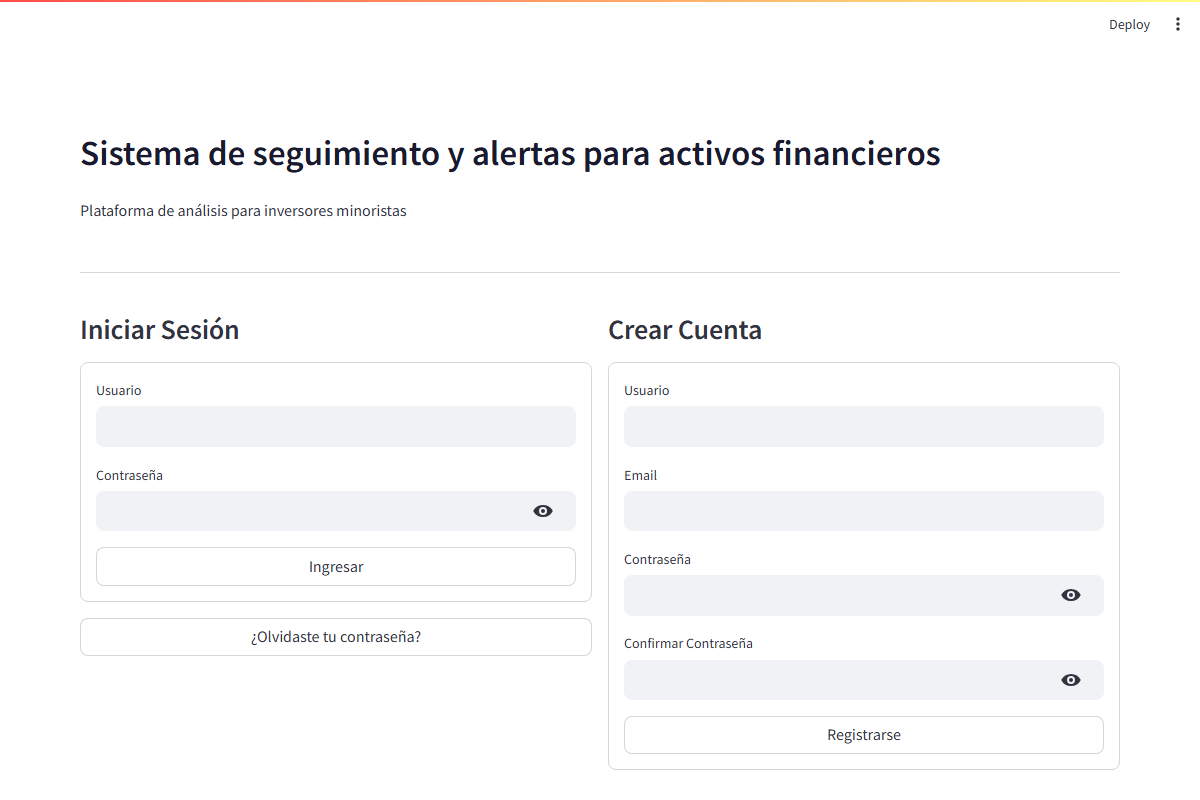
\includegraphics[width=0.85\textwidth]{docs/captura_login.png}
    \caption{Pantalla principal del dashboard Streamlit: formulario de autenticación e inicio de sesión.}
    \label{fig:captura-login}
\end{figure}

La comunicación entre el dashboard y el backend se articula en torno a tres endpoints principales, cuyo flujo se esquematiza en la Figura~\ref{fig:flujo-streamlit-backend}. El proceso inicia con el formulario de login, que envía las credenciales al endpoint \texttt{POST /auth/login} y almacena el token JWT resultante en la sesión de Streamlit. Las solicitudes de predicción se canalizan a \texttt{GET /predict/\{ticker\}}, autenticadas mediante ese token, y retornan el análisis completo del activo. El histórico de alertas se recupera desde \texttt{GET /alerts}, también con autenticación Bearer.

\begin{figure}[H]
    \centering
    \begin{tikzpicture}[
        node distance=12mm and 20mm,
        box/.style={
            rectangle,
            draw,
            rounded corners=2mm,
            align=center,
            inner sep=5pt,
            minimum width=38mm,
            minimum height=10mm,
            font=\small,
            thick
        },
        arrow/.style={-Latex, thick},
        lbl/.style={font=\scriptsize, fill=white, inner sep=1pt}
    ]

    % Nodos del dashboard (izquierda)
    \node[box] (login_ui)  {Formulario\\de login};
    \node[box, below=18mm of login_ui]  (pred_ui)  {Pestaña\\Predicción};
    \node[box, below=18mm of pred_ui]   (alert_ui) {Pestaña\\Alertas};
    \node[above=5mm of login_ui,  font=\small\bfseries] {Dashboard (Streamlit)};

    % Endpoints del backend (derecha)
    \node[box] (login_ep)  at ([xshift=72mm]login_ui)  {\texttt{POST /auth/login}};
    \node[box] (pred_ep)   at ([xshift=72mm]pred_ui)   {\texttt{GET /predict/\{ticker\}}};
    \node[box] (alert_ep)  at ([xshift=72mm]alert_ui)  {\texttt{GET /alerts}};
    \node[above=5mm of login_ep,  font=\small\bfseries] {Backend (FastAPI)};

    % Flujo login
    \draw[arrow] ([yshift= 2pt]login_ui.east)  -- node[lbl,above]{credenciales}      ([yshift= 2pt]login_ep.west);
    \draw[arrow] ([yshift=-2pt]login_ep.west)  -- node[lbl,below]{token JWT}         ([yshift=-2pt]login_ui.east);

    % Flujo predicción
    \draw[arrow] ([yshift= 2pt]pred_ui.east)   -- node[lbl,above]{ticker + Bearer}   ([yshift= 2pt]pred_ep.west);
    \draw[arrow] ([yshift=-2pt]pred_ep.west)   -- node[lbl,below]{análisis completo} ([yshift=-2pt]pred_ui.east);

    % Flujo alertas
    \draw[arrow] ([yshift= 2pt]alert_ui.east)  -- node[lbl,above]{Bearer token}      ([yshift= 2pt]alert_ep.west);
    \draw[arrow] ([yshift=-2pt]alert_ep.west)  -- node[lbl,below]{lista de alertas}  ([yshift=-2pt]alert_ui.east);

    \end{tikzpicture}
    \caption{Flujo de comunicación entre el dashboard Streamlit y los tres endpoints principales del backend.}
    \label{fig:flujo-streamlit-backend}
\end{figure}


\section{Base de datos}

La solución utiliza una base de datos relacional ligera, basada en SQLite,
adecuada para proyectos de prototipo y entornos de laboratorio. La elección de
SQLite responde a consideraciones de simplicidad de despliegue, portabilidad y
ausencia de requerimientos de infraestructura adicional, sin dejar de cumplir
con los requisitos de persistencia, integridad referencial y trazabilidad
necesarios para el análisis posterior.

El acceso a la base se realiza a través de SQLAlchemy, que permite definir los
modelos de datos mediante clases de Python mapeadas a tablas mediante el patrón
ORM. Entre las tablas principales se encuentran las correspondientes a usuarios,
alertas, métricas de modelos y tokens de recuperación de contraseña. Cada tabla
fue diseñada para capturar únicamente la información necesaria para el
funcionamiento del sistema y la posterior auditoría de sus decisiones.

La tabla~\ref{tab:usuarios} presenta la estructura de la tabla de usuarios, que
almacena la identificación, el nombre de usuario, el correo electrónico (en caso
de estar disponible), la contraseña cifrada, el rol asignado y la fecha de
registro. Este diseño permite diferenciar entre administradores y analistas, lo
que facilita la implementación de controles de acceso basados en roles en una
etapa posterior.

\begin{table}[h]
\centering
\caption{Estructura de la tabla \texttt{usuarios}.}
\label{tab:usuarios}
\begin{tabular}{lll}
\toprule
\textbf{Campo} & \textbf{Tipo} & \textbf{Descripción} \\
\midrule
\texttt{id}               & INTEGER (PK) & Identificador único del usuario. \\
\texttt{username}         & TEXT         & Nombre de usuario para autenticación. \\
\texttt{email}            & TEXT         & Correo electrónico asociado (opcional). \\
\texttt{password\_hash}   & TEXT         & Hash seguro de la contraseña (bcrypt). \\
\texttt{rol}              & TEXT         & Rol asignado (admin, \analista ). \\
\texttt{fecha\_creacion}  & DATETIME     & Fecha y hora de registro del usuario. \\
\bottomrule
\end{tabular}
\end{table}

La tabla~\ref{tab:alertas} resume la estructura de la tabla de alertas, en la
que se registra para cada evento el identificador interno, el usuario asociado,
el ticker afectado, el tipo de severidad, un mensaje descriptivo, la
variación porcentual prevista, los precios actual y proyectado, el estado de
lectura y la marca de tiempo de creación. Este registro posibilita reconstruir,
para cualquier activo y período, qué eventos fueron considerados relevantes por
el sistema y con qué intensidad.

\begin{table}[h]
\centering
\caption{Estructura de la tabla \texttt{alertas}.}
\label{tab:alertas}
\begin{tabular}{lll}
\toprule
\textbf{Campo} & \textbf{Tipo} & \textbf{Descripción} \\
\midrule
\texttt{id}               & INTEGER (PK) & Identificador interno de la alerta. \\
\texttt{usuario\_id}      & INTEGER (FK) & Usuario asociado a la alerta. \\
\texttt{ticker}           & TEXT         & Activo financiero que originó la alerta. \\
\texttt{tipo}             & TEXT         & Nivel de severidad \\
\texttt{mensaje}          & TEXT         & Descripción de la alerta generada. \\
\texttt{variacion\_pct}   & REAL         & Variación porcentual esperada. \\
\texttt{precio\_actual}   & REAL         & Precio de mercado actual \\
\texttt{precio\_predicho} & REAL         & Precio proyectado por el modelo. \\
\texttt{leida}            & INTEGER      & 0~=~no leída, 1~=~leída. \\
\texttt{fecha\_creacion}  & DATETIME     & Momento de creación de la alerta. \\
\bottomrule
\end{tabular}
\end{table}

La tabla~\ref{tab:metricas} muestra la estructura de la tabla de métricas de
modelo, que registra el desempeño del clasificador binario en cada predicción.
Dado que el modelo predice la dirección del precio (SUBIDA/BAJADA), las métricas
almacenadas son propias de clasificación: exactitud general (Accuracy),
precisión y recall sobre la clase positiva (SUBIDA), su balance armónico
(F1-Score) y el área bajo la curva ROC (AUC-ROC). De esta manera, es posible
monitorear la evolución temporal de la capacidad discriminativa del modelo e
identificar posibles degradaciones debidas a cambios estructurales en el mercado.

\begin{table}[h]
\centering
\caption{Estructura de la tabla \texttt{metricas\_modelo}.}
\label{tab:metricas}
\begin{tabular}{lll}
\toprule
\textbf{Campo} & \textbf{Tipo} & \textbf{Descripción} \\
\midrule
\texttt{id}           & INTEGER (PK)   & Identificador único del registro de métrica. \\
\texttt{usuario\_id}  & INTEGER (FK)   & Usuario que ejecutó la predicción (opcional). \\
\texttt{ticker}       & VARCHAR(20)    & Símbolo del activo financiero analizado. \\
\texttt{modelo}       & VARCHAR(50)    & Nombre del modelo utilizado (por defecto: \texttt{ensemble\_clasificador}). \\
\texttt{accuracy}     & REAL           & Exactitud general del clasificador (Accuracy). \\
\texttt{precision}    & REAL           & Precisión de clase positiva, SUBIDA (Precision). \\
\texttt{recall}       & REAL           & Sensibilidad de clase positiva, SUBIDA (Recall). \\
\texttt{f1}           & REAL           & Balance entre precisión y recall (F1-Score). \\
\texttt{auc}          & REAL           & Área bajo la curva ROC (AUC-ROC). \\
\texttt{fecha}        & DATETIME       & Fecha y hora del registro (por defecto: UTC actual). \\
\bottomrule
\end{tabular}
\end{table}

El esquema incluye además una tabla auxiliar \texttt{password\_reset\_tokens},
que almacena los tokens temporales generados durante el flujo de recuperación
de contraseña. Cada token está vinculado a un usuario mediante clave foránea,
registra su fecha de expiración y un indicador de uso, garantizando que cada
token pueda emplearse una única vez.




La figura~\ref{fig:er-db} sintetiza la estructura global de la base de datos mediante un diagrama entidad–relación que ilustra, de forma directa, cómo interactúan los elementos centrales del sistema. En este modelo, la entidad usuarios se vincula con la entidad métricas mediante una relación 1:N, lo que indica que cada usuario puede poseer múltiples registros de desempeño del modelo. A su vez, métricas se relaciona con alertas también mediante una relación 1:N, reflejando que cada evaluación del modelo puede dar origen a una o varias alertas registradas.

Este encadenamiento estructural permite reconstruir, para cualquier alerta emitida, qué métrica del modelo la generó y a qué usuario pertenece dicha métrica, lo que garantiza la  trazabilidad completa para auditorías, análisis posteriores y explicabilidad. El esquema ER, complementado con las tablas detalladas de campos, tipos de datos y claves primarias/foráneas, constituye así la documentación técnica fundamental para la evolución futura del sistema y permite extender la base de datos  ( o integrarla con otros módulos) de manera controlada, consistente y verificable.

\begin{figure}[H]
\centering
\begin{tikzpicture}[
    entity/.style={
        draw,
        rounded corners=3pt,
        align=center,
        minimum width=32mm,
        minimum height=8mm,
        font=\small
    },
    rel/.style={
        font=\small,
        fill=white,
        inner sep=1pt
    },
    node distance=18mm,
    arrow/.style={-Latex, thick}
]

% Entidades
\node[entity] (usuarios) {usuarios};
\node[entity, below=of usuarios] (metricas) {métricas};
\node[entity, below=of metricas] (alertas) {alertas};

% Flechas con etiquetas 1:N sobre la línea
\draw[arrow] (usuarios) -- node[rel, right]{1 : N} (metricas);
\draw[arrow] (metricas) -- node[rel, right]{1 : N} (alertas);

\end{tikzpicture}

\caption{Diagrama entidad–relación de la base de datos.}
\label{fig:er-db}
\end{figure}


\section{Sistema de alertas}



El sistema de alertas constituye el componente más visible para el usuario cuando
se superan ciertos umbrales de riesgo o se detectan escenarios potencialmente
críticos. El flujo se inicia en el endpoint de predicción: una vez finalizado el
cálculo, el backend evalúa, junto con el agente de alertas, si el cambio porcentual
previsto para el activo y la señal de mercado justifican la creación de una
notificación.

El sistema integra un canal de notificación que es la consulta   \texttt {REST al endpoint /alerts/}. A través de este canal , el dashboard recupera y presenta las alertas persistidas en la base de datos.
La   integración de notificaciones push mediante WebSocket y el envío de correo electrónico ante  alertas críticas quedan propuestos como trabajo futuro.

El agente de alertas evalúa de forma continua los resultados de predicción y los
indicadores de sentimiento. Cuando la magnitud del cambio porcentual esperado
supera umbrales previamente definidos, se genera una advertencia o una alerta
crítica, según la severidad del movimiento. La figura~\ref{fig:flujo-alertas}
resume este proceso desde la obtención del resultado de predicción hasta el envío
de la notificación al usuario para las acciones de APPLE.


\begin{figure}[H]
  \centering
  \begin{adjustbox}{center}
  \begin{tikzpicture}[
      xshift=-6mm,
      node distance=14mm,
      box/.style={
          draw,
          rounded corners=2mm,
          align=center,
          inner sep=4pt,
          minimum width=45mm,
          minimum height=10mm,
          font=\small
      },
      arrow/.style={-Latex, thick}
  ]

  % Nodos en vertical
  \node[box] (pred) {Resultado de predicción\\(cambio \% previsto, sentimiento)};
  \node[box, below=of pred] (eval) {Evaluación de anomalías};
  \node[box, below=of eval] (adv) {APPLE\\(Advertencia)};
  \node[box, below=of adv] (crit) {Alerta crítica};
  \node[box, below=of crit] (bd) {Registro en base de datos};
  \node[box, below=of bd] (rest) {Consulta REST\\(dashboard)};

  % Flechas verticales
  \draw[arrow] (pred.south) -- (eval.north);
  \draw[arrow] (eval.south) -- (adv.north);
  \draw[arrow] (adv.south) -- (crit.north);
  \draw[arrow] (crit.south) -- (bd.north);
  \draw[arrow] (bd.south) -- (rest.north);

  \end{tikzpicture}
  \end{adjustbox}

  \caption{Diagrama vertical del flujo de generación y consulta de alertas.}
  \label{fig:flujo-alertas}
  \end{figure}

En el prototipo actual, el criterio de decisión combina múltiples técnicas de detección de 
  anomalías: Z-Score, MAD (Median Absolute Deviation), CUSUM para cambios de tendencia, EWMA  
  para control estadístico e Isolation Forest para anomalías multivariadas. El resultado      
  integrado de estos detectores determina uno de seis niveles de severidad: INFO, LOW, MEDIUM,   HIGH, CRITICAL y EMERGENCY. 
  
  El sistema distingue además nueve tipos de alerta: movimiento  
  de precio, pico de volatilidad, cambio de tendencia, anomalía detectada, volumen inusual,   
  cambio de sentimiento, divergencia de predicción, ruptura de correlación y patrón detectado.   Estos parámetros pueden ajustarse según el perfil de riesgo del usuario y la volatilidad   
  típica de los activos bajo análisis.
  
Una vez tomada la decisión, el agente de alertas construye un registro con los campos definidos en la base de datos    
  (usuario, activo, tipo, mensaje, variación prevista, precio actual, precio predicho y       
  fecha)y lo persiste en la tabla correspondiente.
  
  La
visualización de las alertas en la interfaz se realiza a través del endpoint de
listado, que recupera los registros más recientes y los presenta en forma de
histórico filtrable. La tabla~\ref{tab:alertas} muestra un ejemplo
simplificado de las alertas que pueden registrarse durante la operación del
sistema para distintos activos financieros.


\begin{table}[H]
\centering
\renewcommand{\arraystretch}{1.15}

\caption{Ejemplo de alertas generadas por movimientos fuera del rango esperado .}
\label{tab:alertas}

\begin{tabularx}{0.98\textwidth}{
    p{2.9cm}   % Fecha y hora
    p{1.4cm}   % Ticker
    X          % Mensaje resumido
    p{1.2cm}   % Variación
    p{2.2cm}   % Canal
}
\toprule
\textbf{Fecha y hora} & \textbf{Ticker} &
\textbf{Mensaje resumido} &
\textbf{Var.\ (\%)} & \textbf{Canal} \\
\midrule

2025-11-03 10:22 & AAPL &
Variación moderada fuera del rango esperado según el modelo (estado APPLE). &
+2.8 & Consulta REST\\

2025-11-03 12:40 & TSLA &
Incremento abrupto en la volatilidad intradía identificado por el sistema. &
-3.4 & Consulta REST \\

2025-11-03 15:10 & NVDA &
Desvío significativo respecto de la tendencia prevista por el modelo predictivo. &
+3.1 & Consulta REST \\

\bottomrule
\end{tabularx}

\end{table}

El sistema implementa un servicio SMTP con autenticación segura, en línea con las
  recomendaciones de seguridad propuestas por OWASP \parencite{owasp2021}, utilizado
  para notificaciones de autenticación: recuperación de contraseña y confirmación de
  cambio de contraseña. El envío de correos ante alertas financieras críticas queda
  propuesto como trabajo futuro.

\section{Seguridad}

 La arquitectura del sistema incorpora un conjunto de mecanismos de seguridad
  orientados a garantizar la integridad de los datos, la confidencialidad de la
  información sensible y la trazabilidad de las operaciones. Estas medidas se
  encuentran alineadas tanto con las buenas prácticas internacionales propuestas
  por OWASP \parencite{owasp2021}, como con los lineamientos establecidos por el
  Banco Central de la República Argentina para la gestión de riesgos informáticos
  \parencite{bcra7724}.

  Entre los mecanismos implementados se destacan:

  \begin{itemize}
      \item Autenticación robusta mediante \textit{JSON Web Tokens} (JWT).
      \item Hash seguro de contraseñas utilizando \texttt{bcrypt}.
      \item Validación estricta de parámetros mediante modelos \texttt{Pydantic}.
      \item Rate limiting de alertas para evitar saturación de notificaciones repetidas por   
  activo.
      \item Registro estructurado de eventos (logging con marca temporal, módulo y nivel de   
  severidad).
  \end{itemize}

  En primera instancia, el sistema implementa un mecanismo de autenticación basado
  en JWT, en el que cada usuario recibe un token firmado digitalmente con una clave
  privada almacenada en variables de entorno. Este token contiene la identidad del
  usuario, información adicional para autorización y una fecha de expiración que
  limita su uso. La validación de los tokens se realiza en cada endpoint protegido,
  lo que reduce así el riesgo de accesos no autorizados.

  Las contraseñas de los usuarios nunca se almacenan en texto plano. El backend
  utiliza la biblioteca \texttt{Passlib} con el algoritmo \texttt{bcrypt}, que
  aplica funciones de hash lentas y resistentes a ataques de fuerza bruta. En caso
  de comprometerse la base de datos, los hashes no pueden revertirse mediante
  técnicas de descifrado directo, cumpliendo con los estándares recomendados por
  OWASP para la protección de credenciales.

  Otro de los pilares del sistema es la validación rigurosa de los datos de entrada.
  FastAPI, apoyado en Pydantic, garantiza que todo parámetro recibido cumple con el
  tipo, formato y restricciones definidas en los modelos. Esto evita procesar
  solicitudes incorrectas, incompletas o manipuladas con intención maliciosa, lo que
  reduce significativamente la superficie de ataque.

  El sistema implementa rate limiting a nivel de generación de alertas, controlando
  la frecuencia con que se emiten notificaciones por activo financiero para evitar
  saturación de alertas repetidas. La limitación de frecuencia sobre los endpoints
  HTTP de la API queda propuesta como trabajo futuro.

  La gestión de secretos del sistema se realiza mediante variables de entorno,
  evitando la inclusión de credenciales directamente en el código fuente. La clave
  secreta utilizada para firmar los tokens JWT, así como los parámetros de conexión
  a la base de datos, se cargan en tiempo de ejecución a través de \texttt{Pydantic
  Settings}, garantizando que información sensible no quede expuesta en repositorios
  de control de versiones ni en artefactos de despliegue.

Finalmente, el sistema incorpora un módulo de auditoría que registra eventos
  con marca temporal, módulo origen y nivel de severidad mediante el módulo
  estándar de logging de Python. Cada operación relevante queda trazada con
  estos parámetros descriptivos, lo que facilita la detección de anomalías, la
  investigación de incidentes y el cumplimiento de los requerimientos regulatorios
  del BCRA para sistemas tecnológicos en instituciones financieras.

La figura~\ref{fig:seguridad-flujo} sintetiza visualmente estas capas de
  protección, mostrando la secuencia de validaciones y controles que intervienen en
  cada solicitud.

  \begin{figure}[H]
  \centering
  \begin{tikzpicture}[
      node distance=12mm,
      box/.style={
          draw,
          rounded corners=2mm,
          align=center,
          inner sep=4pt,
          minimum width=46mm,
          minimum height=10mm,
          font=\small
      },
      arrow/.style={-Latex, thick}
  ]

  \node[box] (auth) {Autenticación\\JWT};
  \node[box, below=of auth] (bcrypt) {Protección de contraseñas\\(\texttt{bcrypt})};
  \node[box, below=of bcrypt] (valid) {Validación de datos\\(\texttt{Pydantic})};
  \node[box, below=of valid] (limit) {Rate limiting de alertas};
  \node[box, below=of limit] (log) {Logging estructurado\\(texto plano)};

  \draw[arrow] (auth) -- (bcrypt);
  \draw[arrow] (bcrypt) -- (valid);
  \draw[arrow] (valid) -- (limit);
  \draw[arrow] (limit) -- (log);

  \end{tikzpicture}
  \caption{Diagrama del flujo de seguridad implementado en el sistema.}
  \label{fig:seguridad-flujo}
  \end{figure}

  La tabla~\ref{tab:seguridad-descriptivo} resume las funciones de cada componente e ilustra  
  cómo contribuyen al modelo integral de seguridad del sistema.
  

  \begin{table}[H]
  \caption{Componentes de seguridad implementados.}
  \label{tab:seguridad-descriptivo}
  \centering
  \renewcommand{\arraystretch}{1.25}
  \begin{tabularx}{0.98\textwidth}{l X}
  \toprule
  \textbf{Componente} & \textbf{Descripción} \\
  \midrule
  Autenticación JWT &
  Controla el acceso a endpoints protegidos mediante tokens firmados que incluyen identidad,  
  permisos y expiración. \\
  \midrule
  Hash \texttt{bcrypt} &
  Protege credenciales aplicando un hash lento y resistente a ataques de fuerza bruta,        
  conforme a OWASP. \\
  \midrule
  Validación de datos &
  Comprueba tipos, formatos y restricciones de todos los parámetros recibidos, evitando       
  entradas malformadas o maliciosas. \\
  \midrule
  Rate limiting de alertas &
  Controla la frecuencia con que se emiten notificaciones por activo financiero, evitando     
  saturación de alertas repetidas. \\
  \midrule
  Logging estructurado &
  Registra acciones relevantes con marca temporal, módulo origen y nivel de severidad para    
  auditoría, detección de anomalías y cumplimiento normativo BCRA. \\
  \bottomrule
  \end{tabularx}
  \end{table}



\section{Pipeline de procesamiento}

El pipeline de procesamiento constituye el eje central del funcionamiento del sistema, ya que define la secuencia lógica mediante la cual los datos brutos son transformados en información procesada, evaluada y finalmente presentada al usuario en forma de predicciones y alertas. Su diseño modular permite que cada etapa funcione de manera independiente y coordinada, favoreciendo la extensibilidad y la incorporación futura de nuevos modelos o fuentes de información.

El flujo completo está compuesto por siete etapas principales:

\begin{enumerate}
    \item Ingesta y validación de datos de mercado.
    \item Normalización y limpieza de series.
    \item Ejecución de modelos predictivos.
    \item Análisis de noticias y sentimiento.
    \item Integración de señales y generación de alertas.
    \item Almacenamiento estructurado en base de datos.
    \item Visualización interactiva en el dashboard.
\end{enumerate}

La modularidad del pipeline permite incorporar nuevos activos, modelos o fuentes de datos sin modificar la estructura base de la arquitectura, dado que cada etapa está encapsulada en un agente especializado y se interconecta mediante el backend.

En primer lugar, se encuentra la etapa de ingesta de datos, en la que el agente de mercado descarga las series históricas del activo seleccionado. Este proceso contempla la comunicación con proveedores externos, la captura de posibles errores de red, la verificación de integridad y la adaptación del formato recibido a la estructura interna del sistema. Solo si los datos superan estas verificaciones se habilita su uso en las etapas siguientes.

Luego se realiza el preprocesamiento y normalización, que incluye selección de columnas relevantes, tratamiento de valores faltantes, ajuste de escalas, conversión de tipos de datos y cálculo de indicadores agregados (por ejemplo, variación porcentual o medias móviles). Este paso resulta fundamental para garantizar que el modelo predictivo trabaje con un conjunto de datos limpio y coherente.

A continuación, en la etapa de modelado, el agente de predicción entrena un  ensemble de clasificadores    (Random Forest, Gradient Boosting, XGBoost y LightGBM) sobre una ventana móvil de
  observaciones recientes. 
  
  Se utiliza  walk-forward validation temporal. Como resultado, el    
  sistema genera una probabilidad de movimiento alcista o bajista para el activo en el        
  horizonte de tres días, acompañada de métricas de clasificación (Accuracy, Precision,       
  Recall, F1-Score y AUC-ROC).

Paralelamente, el agente de sentimiento consulta noticias recientes del activo
  mediante Yahoo Finance y las analiza con un ensemble de cuatro modelos: FinBERT
  (40\%), VADER (25\%), TextBlob (15\%) y un lexicón financiero propio de más de
  500 términos (20\%). El resultado es una señal cualitativa que complementa la
  información cuantitativa del modelo predictivo.

  La siguiente fase corresponde a la integración y recomendación. El agente de
  recomendación combina la predicción cuantitativa, la señal de mercado y la
  información de sentimiento para generar un mensaje comprensible para el usuario.
  Sobre esta base se ejecuta la evaluación de alertas, en la que el agente
  correspondiente determina el nivel de severidad (INFO, LOW, MEDIUM, HIGH, CRITICAL
  o EMERGENCY) mediante técnicas estadísticas de detección de anomalías, y persiste
  el registro en la base de datos para su consulta desde el dashboard.

  Finalmente, los resultados se persisten en la base de datos junto con su marca
  temporal, lo que permite la auditoría y trazabilidad. La API devuelve la
  información en formato JSON, facilitando que el dashboard de Streamlit visualice
  predicciones, métricas y alertas.

  
La figura~\ref{fig:pipeline-vertical} muestra una representación vertical del pipeline, en la que se destaca el rol de cada agente y la secuencia de transformación de los datos hasta su presentación final al usuario.

\begin{figure}[H]
\centering
\begin{tikzpicture}[
    node distance=12mm,
    box/.style={
        draw,
        rounded corners=2mm,
        align=center,
        inner sep=4pt,
        minimum width=48mm,
        minimum height=10mm,
        font=\small
    },
    arrow/.style={-Latex, thick}
]

% NODOS PRINCIPALES DEL PIPELINE
\node[box] (ingesta) {Ingesta de datos\\(Agente de mercado)};
\node[box, below=of ingesta] (prep) {Normalización y limpieza\\de series temporales};
\node[box, below=of prep] (modelo) {Ejecución de modelo\\predictivo};
\node[box, below=of modelo] (sent) {Análisis de noticias\\y sentimiento};
\node[box, below=of sent] (reco) {Integración y\\generación de alertas};
\node[box, below=of reco] (bd) {Registro en base de datos};
\node[box, below=of bd] (viz) {Visualización\\en dashboard};

% FLECHAS
\draw[arrow] (ingesta) -- (prep);
\draw[arrow] (prep) -- (modelo);
\draw[arrow] (modelo) -- (sent);
\draw[arrow] (sent) -- (reco);
\draw[arrow] (reco) -- (bd);
\draw[arrow] (bd) -- (viz);

\end{tikzpicture}

\caption{Diagrama vertical del pipeline completo de procesamiento, desde la ingesta hasta la visualización.}
\label{fig:pipeline-vertical}
\end{figure}



\section{Despliegue y entorno}

  El sistema se despliega utilizando:

  \begin{itemize}
      \item Archivos \texttt{requirements.txt} para gestionar dependencias.
      \item Servidores ASGI (Uvicorn) para ejecución del backend.
      \item Variables de entorno para claves sensibles.
  \end{itemize}

  Esta estrategia garantiza que las pruebas locales sean reproducibles y
  fácilmente transportables entre equipos de trabajo.

  El backend se distribuye junto con un archivo \texttt{requirements.txt} que
  declara las dependencias de Python necesarias para su ejecución, incluyendo
  \texttt{FastAPI, Uvicorn, SQLAlchemy, Pydantic}, las bibliotecas de seguridad
  y los paquetes para tratamiento de datos.

  La configuración sensible, como claves secretas y cadenas de conexión a la
  base de datos, se gestiona a través de variables de entorno definidas en un
  archivo \texttt{.env}. La clase de configuración del backend, basada en
  \texttt{Pydantic Settings}, se encarga de cargar estos valores y ponerlos a
  disposición del resto de la aplicación sin que queden expuestos en el código
  fuente.

  Para la ejecución local, el servidor se activa mediante Uvicorn, un servidor
  ASGI ligero. De esta manera, es posible probar la API en un entorno de
  desarrollo con una simple instrucción de consola. La misma configuración puede
  adaptarse a entornos de producción aumentando el número de trabajadores o
  integrando el servicio en un servidor web más robusto.

  La estructura de carpetas y la separación entre backend y dashboard facilita
  la creación futura de imágenes Docker independientes (por ejemplo, una para
  la API y otra para la interfaz de usuario), lo que queda propuesto como
  trabajo futuro.

  
La tabla~\ref{tab:dependencias} resume las principales 
bibliotecas utilizadas, su propósito dentro del sistema y su tipo de funcionalidad.

\begin{longtable}{p{2.5cm} p{2.3cm} p{6.5cm}}
  \caption{Bibliotecas principales}
  \label{tab:dependencias} \\

  \toprule
  \textbf{Paquete} & \textbf{Categoría} & \textbf{Función dentro del sistema} \\
  \midrule
  \endfirsthead

  \multicolumn{3}{c}{\tablename\ \thetable{} -- continuación} \\
  \toprule
  \textbf{Paquete} & \textbf{Categoría} & \textbf{Función dentro del sistema} \\
  \midrule
  \endhead

  \midrule
  \multicolumn{3}{r}{\textit{Continúa en la página siguiente}} \\
  \endfoot

  \bottomrule
  \endlastfoot

  \texttt{fastapi} & Backend API &
  Framework principal para definir endpoints, validar datos y generar documentación OpenAPI.  
  \\
  \midrule

  \texttt{uvicorn} & Servidor ASGI &
  Ejecuta la aplicación FastAPI y permite un manejo concurrente y despliegue liviano. \\      
  \midrule

  \texttt{pydantic} & Validación &
  Modelado estricto de datos y carga segura de variables de entorno mediante
  \texttt{pydantic-settings}. \\
  \midrule

  \texttt{sqlalchemy} & Base de datos &
  ORM para definir modelos, manejar sesiones y ejecutar consultas sobre SQLite. \\
  \midrule

  \texttt{passlib} & Seguridad &
  Hash seguro de contraseñas con \texttt{bcrypt}, resistente a ataques de fuerza bruta según  
  OWASP. \\
  \midrule

  \texttt{python-jose} & Seguridad &
  Generación y validación de tokens JWT para autenticación de usuarios. \\
  \midrule

  \texttt{yfinance} & Datos financieros &
  Descarga de series históricas de precios y noticias recientes de activos desde Yahoo        
  Finance. \\
  \midrule

  \texttt{pandas} & Procesamiento &
  Limpieza, manipulación y normalización de series históricas de precios. \\
  \midrule

  \texttt{numpy} & Cálculo numérico &
  Soporte matemático para operaciones vectorizadas y cálculo de indicadores técnicos. \\      
  \midrule

  \texttt{ta} & Análisis técnico &
  Cálculo de más de 20 indicadores técnicos (RSI, MACD, Bollinger Bands, ATR, OBV, entre      
  otros). \\
  \midrule

  \texttt{scikit-learn} & Modelado &
  Clasificadores base (Random Forest, Gradient Boosting), preprocesamiento y métricas de      
  clasificación. \\
  \midrule

  \texttt{xgboost} & Modelado &
  Clasificador XGBoost para predicción binaria de dirección de precios, parte del ensemble. \\  \midrule

  \texttt{lightgbm} & Modelado &
  Clasificador LightGBM para predicción binaria de dirección de precios, parte del ensemble.  
  \\
  \midrule

  \texttt{torch} & Deep Learning &
  Implementación opcional del modelo LSTM para predicción de series temporales. \\
  \midrule

  \texttt{transformers} & NLP &
  Carga del modelo FinBERT (ProsusAI/finbert) para análisis de sentimiento financiero. \\     
  \midrule

  \texttt{nltk} & NLP &
  Análisis de sentimiento mediante VADER, optimizado para textos de redes sociales y noticias.   \\
  \midrule

  \texttt{textblob} & NLP &
  Análisis de polaridad general de texto, componente del ensemble de sentimiento. \\
  \midrule

  \texttt{streamlit} & Dashboard &
  Interfaz de usuario interactiva para visualización de predicciones, métricas y alertas. \\  
  \midrule

  \texttt{plotly} & Visualización &
  Gráficos interactivos de precios históricos y predicciones en el dashboard. \\
  \midrule

  \texttt{python-dotenv} & Configuración &
  Carga de variables de entorno desde el archivo \texttt{.env} sin exponer credenciales en el 
  código. \\
  \midrule

  \texttt{smtplib} (estándar) & Notificaciones &
  Envío de correos de recuperación y confirmación de cambio de contraseña mediante SMTP       
  autenticado. \\

  \end{longtable}


\section{Monitoreo y logging}

 El último componente del sistema es el módulo de monitoreo y logging, que tiene
  como finalidad registrar de manera sistemática los eventos relevantes y
  proporcionar información útil para la detección temprana de problemas.

  El módulo registra:

  \begin{itemize}
      \item Errores y excepciones.
      \item Tiempos de respuesta por endpoint.
      \item Frecuencia y severidad de alertas.
  \end{itemize}

  El uso de logging estructurado facilita auditorías completas y permite detectar
  anomalías comportamentales en fases tempranas, reforzando la robustez operativa
  del sistema.

  Cada vez que se ejecutan operaciones clave, como la emisión de una predicción o
  el listado de alertas, se genera un registro con marca de tiempo, nivel de
  severidad, módulo origen y un mensaje descriptivo. Estos registros se visualizan
  en la consola mediante el módulo estándar de logging de Python, y pueden
  redirigirse fácilmente a archivos de log o sistemas centralizados de monitoreo
  en versiones futuras.

El monitoreo del tiempo de respuesta de los endpoints, la frecuencia de llamadas a la API y la tasa de generación de alertas pueden incorporarse en futuras iteraciones del trabajo mediante la integración con soluciones como Prometheus o servicios equivalentes. La información recabada no solo es útil desde el punto de vista técnico, sino que también contribuye a demostrar el cumplimiento de buenas prácticas operativas y de requisitos regulatorios vinculados con el seguimiento de sistemas automatizados en el ámbito financiero.

En conjunto, la arquitectura multiagente, el backend, la interfaz de usuario, la base de datos, el sistema de alertas, los mecanismos de seguridad, el pipeline de procesamiento, el entorno de despliegue y las capacidades de monitoreo conforman una solución integrada que concreta, en un prototipo funcional, los objetivos planteados para el trabajo final.


